% =====================================================================
% GenAI Seminar — A Comparative Study of Autoencoder-Based Generative
% Models for One-Class Anomaly Detection
% Compile on Overleaf (https://overleaf.com): New Project -> Upload, drop
% this file in. No local LaTeX install needed. Put the PNGs you want into a
% figures/ folder (see \includegraphics paths below).
%
% AUTHORING MAP:
%   [P1] = Nicolás (done / drafted)   [P2] = VAE owner   [P3] = AAE owner
% Search for [P2] and [P3] to find the sections each teammate must write.
% =====================================================================
\documentclass[11pt]{article}
\usepackage[margin=1in]{geometry}
\usepackage{graphicx}
\usepackage{booktabs}
\usepackage{amsmath}
\usepackage{amssymb}
\usepackage{hyperref}
\usepackage{caption}

\title{A Comparative Study of Autoencoder-Based Generative Models\\
for One-Class Anomaly Detection}
\author{Nico Dieste Espa\~na \and Claudio Esteban Arambula Delgado \and Andr\'es Campoy Sebasti\'an\\
\small University of Oldenburg --- Generative AI Seminar}
\date{July 2026}

\begin{document}
\maketitle

\begin{abstract}
% [P1 draft — revise once all results are in]
We study unsupervised anomaly detection, where a model is trained only on
normal data and must flag anomalous samples at test time. Rather than contrasting
unrelated model families, we investigate a single, coherent question: \emph{how
does the way a model regularizes its latent space affect anomaly detection?} We
compare three autoencoder-based generative models that form a spectrum of
increasingly explicit latent-space regularization: a plain convolutional
autoencoder (AE, no latent constraint), a variational autoencoder (VAE, a KL
term pulling the latent toward a Gaussian prior), and an adversarial autoencoder
(AAE, an adversarial game matching the latent to that prior). All three share the
same encoder--decoder backbone, are scored by reconstruction error, and are
evaluated under one protocol on a one-class reformulation of Fashion-MNIST and on
the MVTec~AD industrial-defect benchmark, using AUROC and PR-AUC. Our AE baseline
attains a mean AUROC of $0.90$ across the ten Fashion-MNIST classes, establishing
a strong reference against which the VAE and AAE are assessed. For the VAE, we
add an explicit KL-regularized latent model and evaluate both deterministic
reconstruction-error scoring and Monte-Carlo reconstruction-probability scoring
under a $\beta$-ablation. The preliminary class-0 VAE run included in the
repository reports AUROC $0.897$ and PR-AUC $0.933$ with reconstruction-error
scoring; these headline numbers should be replaced by the final
\texttt{scripts/run\_vae\_ablation.py} output once the full run is completed.
The AAE integrates adversarial latent regularization into the same reconstruction-based pipeline and remains competitive, reaching AUROC $0.897$ on the shared setup. Across the three models the differences in AUROC are within roughly one percentage point, indicating that latent-space regularization is approximately neutral for reconstruction-based scoring on this benchmark.
\end{abstract}

% =====================================================================
\section{Introduction}   % [P1 — drafted]
% =====================================================================
Anomaly detection is the task of identifying data points that deviate from a
notion of ``normal.'' It matters wherever anomalies are rare, costly, and hard
to enumerate in advance --- industrial quality control, medical screening,
fraud and intrusion detection. The defining difficulty is asymmetry: normal
data is abundant, whereas anomalies are scarce, diverse, and often unknown at
training time. This makes ordinary supervised classification ill-suited and
motivates a \emph{one-class} approach: learn the structure of normal data alone,
then treat poorly-fitting samples as anomalous.

Autoencoders are a natural fit: trained to compress and reconstruct normal data,
they reconstruct unfamiliar inputs poorly, and the reconstruction error becomes
an anomaly score. But a plain autoencoder places no constraint on its latent
space, which can let it generalize too well and reconstruct anomalies it should
reject. This motivates \emph{regularizing the latent representation}. In this
work we ask a focused question: \emph{does shaping the latent space toward a
known prior improve reconstruction-based anomaly detection, and does the way we
enforce that prior matter?} We study three autoencoder-based models that answer
``how to enforce the prior'' differently, forming a clean progression:
\[
\underbrace{\text{AE}}_{\text{no latent constraint}}
\;\longrightarrow\;
\underbrace{\text{VAE}}_{\text{KL to a Gaussian prior}}
\;\longrightarrow\;
\underbrace{\text{AAE}}_{\text{adversarial match to a prior}} .
\]
By fixing the dataset, the preprocessing, the encoder--decoder backbone, the
scoring convention, and the metrics, we isolate the single variable of interest:
the latent-regularization strategy.

Our contributions are: (i) a unified, reproducible evaluation framework in which
any one-class autoencoder is scored identically; (ii) a strong AE baseline
characterized across all Fashion-MNIST classes; and (iii) a controlled
comparison of AE, VAE, and AAE on Fashion-MNIST and MVTec~AD that reads latent
regularization as the explanatory factor.

% =====================================================================
\section{Related Work}   % [P1 — drafted, ~half a page; add citations]
% =====================================================================
Reconstruction-based anomaly detection with autoencoders is long established:
a network trained to compress and reconstruct normal data fails to reconstruct
unfamiliar inputs, and the reconstruction error serves as an anomaly score.
Variational autoencoders \cite{kingma2013} add a probabilistic latent space,
regularized by a KL term toward a Gaussian prior, and enable likelihood-style
scores; the \emph{reconstruction probability} of An and Cho \cite{ancho2015} is a
widely used VAE anomaly score. Adversarial autoencoders \cite{makhzani2015}
replace the analytic KL term with an adversarial objective: a discriminator,
trained with the adversarial principle of Goodfellow et~al.\ \cite{goodfellow2014},
forces the aggregated posterior of the encoder to match an arbitrary prior. This
places the three models on a single axis --- no constraint, an explicit
divergence, and an adversarial match --- of how strongly and by what mechanism
the latent space is regularized. The MVTec~AD benchmark \cite{bergmann2019}
standardized evaluation on real industrial defects.
In this spectrum, the VAE is the explicit-divergence model: it descends from
variational inference and turns latent regularization into a closed-form KL
penalty, while reconstruction probability extends the VAE objective into an
anomaly score based on the likelihood of reconstructing the input.

% =====================================================================
\section{Background and Methods}
% =====================================================================
\subsection{Problem formulation}   % [P1 — drafted]
Let $\mathcal{X}_{\text{train}}$ contain only normal samples. We train each
model on $\mathcal{X}_{\text{train}}$ and define a scoring function
$s(x)\in\mathbb{R}$ such that higher values indicate more anomalous inputs. At
test time we apply $s$ to a mixed set of normal and anomalous samples and
evaluate ranking quality with threshold-free metrics (Section~4). All three
models share the same encoder $f_\theta$ and decoder $g_\phi$ and use the same
reconstruction-error score
$s(x)=\tfrac{1}{d}\lVert x-g_\phi(f_\theta(x))\rVert_2^2$,
so any difference in performance is attributable to how the latent space is
regularized, not to the score or the architecture.

\subsection{Autoencoder baseline}   % [P1 — drafted]
The autoencoder minimizes reconstruction error on normal data,
$\mathcal{L}_{\text{AE}}=\mathbb{E}_x\lVert x-g_\phi(f_\theta(x))\rVert_2^2$,
with no constraint on the latent code $z=f_\theta(x)$. We use a convolutional
encoder/decoder (two stride-2 conv layers, a 32-dimensional bottleneck, mirrored
transposed convolutions); see the repository for exact layers. This is the
zero-regularization end of the spectrum and the reference the other two must beat.


\subsection{Variational Autoencoder}   % [P2]
The variational autoencoder (VAE) is the explicit-divergence point in our
latent-regularization spectrum. Unlike the plain AE, which maps an input image
$x$ to a single deterministic latent code, the VAE encoder predicts the
parameters of an approximate posterior distribution
$q_{\phi}(z\mid x)=\mathcal{N}(\mu_{\phi}(x),\operatorname{diag}(\sigma^2_{\phi}(x)))$.
The decoder then models the probability of reconstructing $x$ from a sampled
latent variable $z$. In our implementation the prior is the standard Gaussian
$p(z)=\mathcal{N}(0,I)$, so the model is trained not only to reconstruct normal
images but also to keep the latent distribution close to this simple prior.

The training objective is the negative evidence lower bound (ELBO):
\begin{equation}
\mathcal{L}_{\text{VAE}}(x)=
-\mathbb{E}_{q_{\phi}(z\mid x)}[\log p_{\theta}(x\mid z)]
+\beta\,D_{\mathrm{KL}}\big(q_{\phi}(z\mid x)\,\|\,p(z)\big).
\end{equation}
The first term is the reconstruction term; it encourages the decoder to rebuild
the input image accurately. The second term is the KL divergence; it explicitly
pulls the posterior latent distribution toward the Gaussian prior. The parameter
$\beta$ controls the strength of this pressure: small values emphasize
reconstruction, while larger values enforce stronger latent-space
regularization. This makes $\beta$ a natural ablation axis for Person~2.

Because sampling from $q_{\phi}(z\mid x)$ is stochastic, the model uses the
reparameterization trick
\begin{equation}
z = \mu_{\phi}(x) + \sigma_{\phi}(x)\odot\epsilon,\qquad
\epsilon\sim\mathcal{N}(0,I).
\end{equation}
This rewrites the random sample as a deterministic function of the encoder
outputs and an external noise variable. As a result, gradients can flow through
$\mu_{\phi}$ and $\sigma_{\phi}$ during backpropagation even though the latent
variable is sampled.

For anomaly detection, we evaluate two VAE scores. The baseline score is the
mean squared reconstruction error using the posterior mean, matching the AE
protocol. The VAE-specific score is the negative Monte-Carlo reconstruction
probability: for each input, we sample several latent variables
$z_l\sim q_{\phi}(z\mid x)$, compute the Bernoulli reconstruction likelihood
$p_{\theta}(x\mid z_l)$, average these likelihoods with a numerically stable
log-sum-exp operation, and use the negative log probability per pixel as the
anomaly score. Higher values indicate that the input is unlikely under the
VAE's learned reconstruction distribution and is therefore more anomalous.

\subsection{Adversarial Autoencoder}   % [P3]
The adversarial autoencoder (AAE) is the adversarial-match point of the
latent-regularization spectrum. It keeps the same encoder $f_\theta$ and decoder
$g_\phi$ as the AE and VAE, but replaces the VAE's analytic KL term with an
adversarial game played entirely in the latent space. A third network, a latent
discriminator $D_\psi$, is trained to distinguish latent vectors sampled from the
prior $p(z)=\mathcal{N}(0,I)$ from the codes $z=f_\theta(x)$ produced by the
encoder, while the encoder is trained to fool it. At equilibrium the encoder's
aggregated posterior matches the prior, achieving the same goal as the VAE's KL
penalty but through a learned critic rather than a closed-form divergence.

Because the discriminator operates only on latent vectors, a code is labelled
``fake'' purely because it originates from the encoder rather than from the prior;
the underlying image $x$ is always real data. Training alternates three updates
per mini-batch. The reconstruction update trains the encoder and decoder to
minimise pixel error,
\begin{equation}
\mathcal{L}_{\text{rec}} = \tfrac{1}{d}\lVert x - g_\phi(f_\theta(x)) \rVert_2^2 .
\end{equation}
The discriminator update trains $D_\psi$ as a binary classifier that scores prior
samples as real and encoded samples as fake,
\begin{equation}
\mathcal{L}_{D} = -\mathbb{E}_{z\sim p(z)}\!\left[\log D_\psi(z)\right]
                  -\mathbb{E}_{x\sim p_{\text{data}}}\!\left[\log\big(1 - D_\psi(f_\theta(x))\big)\right].
\end{equation}
Finally the adversarial encoder update trains the encoder to make its codes look
prior-like to the discriminator, $\mathcal{L}_{\text{adv}} =
-\mathbb{E}_{x\sim p_{\text{data}}}[\log D_\psi(f_\theta(x))]$, so the encoder's
combined objective is $\mathcal{L}_{\text{AAE}} = \mathcal{L}_{\text{rec}} +
\lambda_{\text{adv}}\,\mathcal{L}_{\text{adv}}$ with a small weight
$\lambda_{\text{adv}}$. As with the AE and VAE, the anomaly score at test time is
the reconstruction error, which keeps the three-way comparison fair. Because the
adversarial game is confined to the low-dimensional latent space rather than the
image space, training is considerably more stable than a full image-space GAN,
though the discriminator and encoder losses should still be monitored. The
architecture is summarised in Figure~\ref{fig:aae_arch}.

\begin{figure}[t]
\centering
% Upload results/figures/aae_architecture.png to figures/
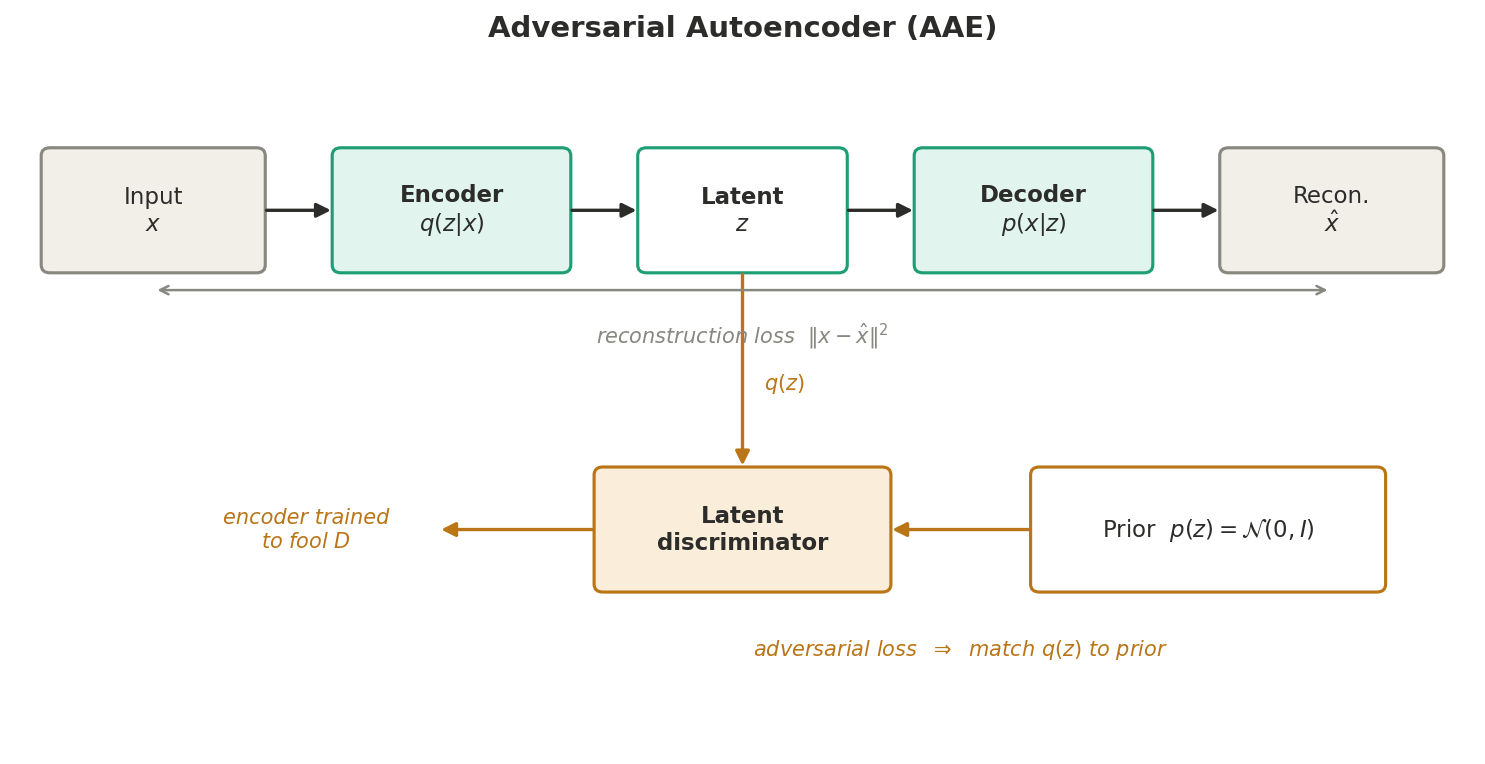
\includegraphics[width=0.85\textwidth]{figures/aae_architecture.png}
\caption{Adversarial autoencoder. The encoder--decoder path (top) is trained for
reconstruction; a latent discriminator (bottom) is trained to separate codes
drawn from the prior $p(z)$ from the encoder's codes $q(z)$, and the encoder is
trained to fool it, driving $q(z)$ toward $p(z)$.}
\label{fig:aae_arch}
\end{figure}

\subsection{The latent-regularization spectrum}   % [P1 — drafted]
The three models differ only in how the latent code is regularized toward a
prior $p(z)=\mathcal{N}(0,I)$: the AE imposes nothing; the VAE adds an analytic
KL divergence $\mathrm{KL}\!\left(q(z|x)\,\|\,p(z)\right)$; and the AAE replaces
that divergence with an adversarial game in which a discriminator matches the
aggregated posterior to $p(z)$. Reading the results along this axis
(Figure~\ref{fig:latent_spectrum}) is the central lens of the paper.

\begin{figure}[t]
\centering
% Upload results/figures/latent_spectrum.png to figures/
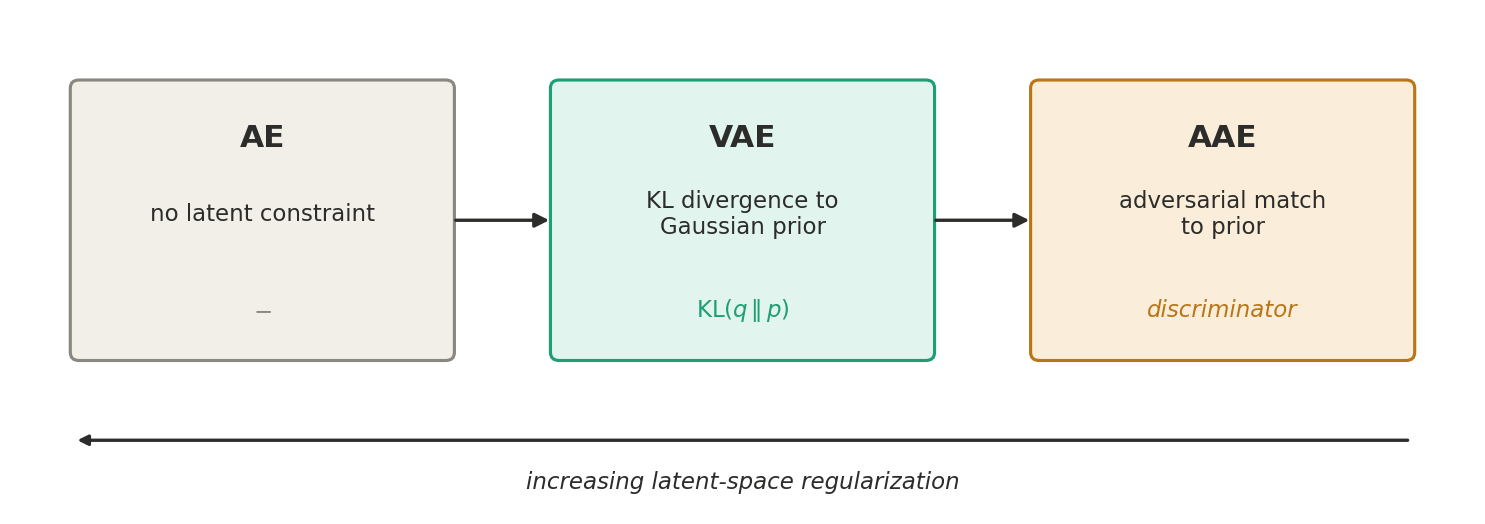
\includegraphics[width=0.9\textwidth]{figures/latent_spectrum.png}
\caption{The three models as a spectrum of latent-space regularization, from no
constraint (AE) to an explicit KL divergence (VAE) to an adversarial match (AAE).}
\label{fig:latent_spectrum}
\end{figure}

\subsection{Implementation and framework}   % [P1 — drafted]
All three models are implemented in PyTorch behind a single interface: each
model exposes \texttt{fit} (train on normal data) and \texttt{anomaly\_score}
(return one score per image, higher $=$ more anomalous). Because the interface
is shared, a common evaluation harness scores every model identically, which is
what makes the comparison fair. The encoder and decoder are shared building
blocks, so the three models use the same backbone (28$\to$14$\to$7 with 64
channels, a 3136-dimensional feature map) and differ only in their latent
treatment and training objective. The framework is reproducible by construction:
a single seeding routine fixes Python, NumPy and PyTorch, the data split is
deterministic, and one command regenerates every table and figure (see the
repository's REPRODUCIBILITY.md).

% =====================================================================
\section{Experimental Setup}   % [P1 — drafted]
% =====================================================================
\paragraph{Datasets.} \emph{Fashion-MNIST} ($28\times28$ grayscale, 10 classes)
is reformulated as one-class anomaly detection: one class is ``normal''
(training and part of the test set) and the other nine are ``anomalies'' in the
test set. \emph{MVTec~AD} provides real industrial images with defect-free
training images and defective test images across 15 categories. Both use the
label convention $0=$ normal, $1=$ anomaly. Dataset documentation (sources,
licenses, preprocessing) is provided as data cards in the repository.

\paragraph{Metrics.} We report the area under the ROC curve (AUROC), which is
threshold-free, and the area under the precision--recall curve (PR-AUC / average
precision), which is more informative when anomalies are rare. Both are computed
over the full mixed test set. As a concrete operating point we additionally
report the best achievable $F_1$ over all thresholds (best-$F_1$), which
summarizes a deployable detector at its optimal threshold.

\paragraph{Training.} All models are trained on normal data only, with the Adam
optimizer and a fixed random seed for reproducibility. Exact hyperparameters and
a one-command reproduction script are in the repository (see REPRODUCIBILITY.md).
Continuous integration runs the unit-test suite on every push, guarding the data
pipeline and the metric computation against regressions.

% =====================================================================
\section{Results}
% =====================================================================
\subsection{Autoencoder baseline across classes}   % [P1 — drafted with real numbers]
Table~\ref{tab:baseline} reports the AE baseline trained separately on each
Fashion-MNIST class (15 epochs each). Mean AUROC is $0.902\pm0.061$ and mean
PR-AUC is $0.939\pm0.041$. Performance is strong for visually distinctive
classes (Trouser $0.99$, Sneaker $0.98$) and weakest for Shirt ($0.80$), which
overlaps heavily with T-shirt, Pullover, and Coat --- an expected and
interpretable failure mode. Figure~\ref{fig:recon} illustrates the mechanism:
trained on T-shirts, the model forces trouser inputs into a shirt-like shape,
producing large, localized reconstruction error.

\begin{table}[t]
\centering
\caption{AE baseline on Fashion-MNIST one-class anomaly detection (15 epochs,
seed 0, 200 anomaly images sampled per non-normal class).}
\label{tab:baseline}
\begin{tabular}{lcc}
\toprule
Normal class & AUROC & PR-AUC \\
\midrule
T-shirt  & 0.9022 & 0.9304 \\
Trouser  & 0.9895 & 0.9928 \\
Pullover & 0.8656 & 0.9149 \\
Dress    & 0.9238 & 0.9537 \\
Coat     & 0.8861 & 0.9349 \\
Sandal   & 0.8784 & 0.9411 \\
Shirt    & 0.7985 & 0.8727 \\
Sneaker  & 0.9794 & 0.9896 \\
Bag      & 0.8264 & 0.8781 \\
Boot     & 0.9728 & 0.9849 \\
\midrule
\textbf{mean $\pm$ std} & \textbf{0.9023 $\pm$ 0.0614} & \textbf{0.9393 $\pm$ 0.0407} \\
\bottomrule
\end{tabular}
\end{table}

\begin{figure}[t]
\centering
% Upload results/baseline_all_classes/ae_reconstructions_class0.png to figures/
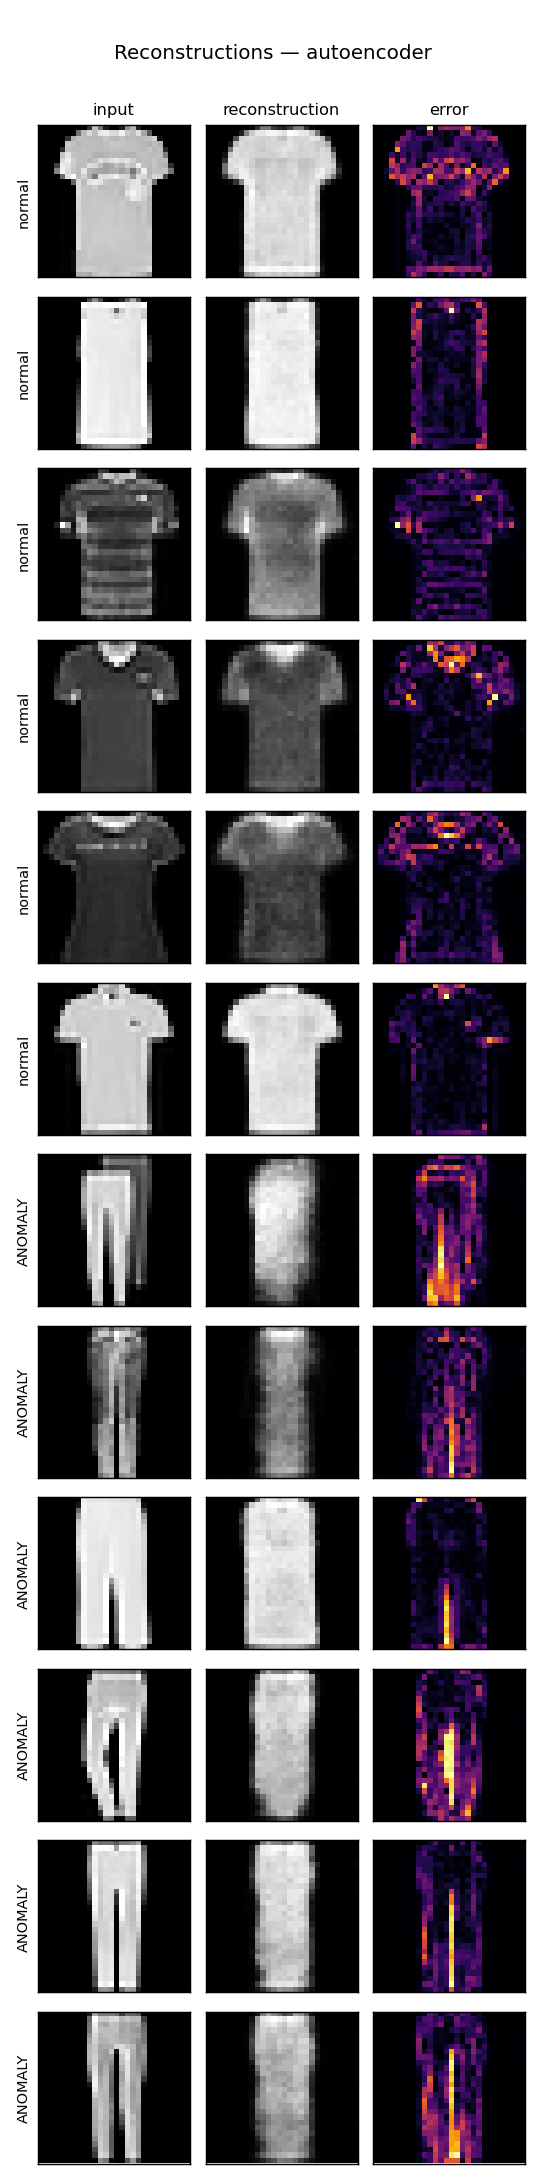
\includegraphics[width=0.5\textwidth]{figures/ae_reconstructions_class0.png}
\caption{AE reconstructions (normal class = T-shirt). Top rows: normal inputs
reconstruct cleanly. Bottom rows: trouser anomalies are forced into a shirt
shape, producing high error (bright regions).}
\label{fig:recon}
\end{figure}

\begin{figure}[t]
\centering
% Upload results/baseline_all_classes/auroc_by_class.png to figures/
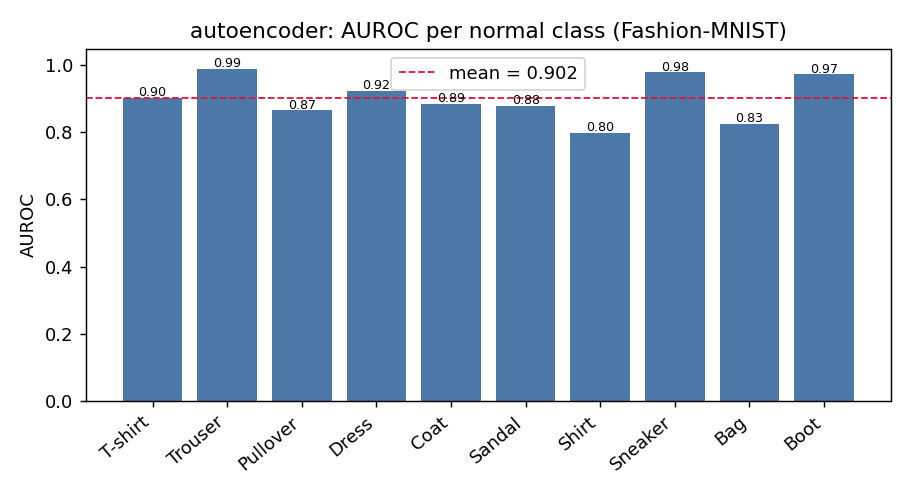
\includegraphics[width=0.75\textwidth]{figures/auroc_by_class.png}
\caption{AE baseline AUROC for each Fashion-MNIST normal class. Performance is
consistently strong (mean $0.90$, dashed line) but varies with how visually
distinctive the normal class is; Shirt is hardest due to overlap with other
tops.}
\label{fig:auroc_class}
\end{figure}


\subsection{VAE results}   % [P2]
Under the shared reconstruction-error scoring protocol, the VAE ($\beta=1$)
obtains AUROC $0.9037$ and PR-AUC $0.9355$ on the class-0 setup
(Table~\ref{tab:comparison}), placing it marginally above the AE baseline but
well within one percentage point --- a difference we do not interpret as a
meaningful improvement.

Beyond this single point, Person~2 evaluates two distinct VAE scores and the role
of the regularization strength. The script \texttt{scripts/run\_vae\_ablation.py}
trains the VAE for $\beta\in\{0.5,1.0,2.0\}$ and scores each trained model with
both the deterministic MSE reconstruction error and the Monte-Carlo
reconstruction-probability score of An and Cho~\cite{ancho2015}, reporting means
and standard deviations across seeds (Table~\ref{tab:vae-beta-ablation}). Two
observations follow. First, under the MSE score the VAE is remarkably robust to
$\beta$: AUROC stays close to $0.90$ across $\beta\in\{0.5,1.0,2.0\}$, with only
small differences that lie within the seed-to-seed standard deviation, so no
single $\beta$ can be declared clearly best on this benchmark. Second, and more
strikingly, the Monte-Carlo reconstruction-probability score performs
substantially \emph{worse} than the simple MSE score (AUROC around $0.52$--$0.62$
versus $\approx0.90$), and it improves as $\beta$ grows. This shows that a more
principled latent-aware likelihood does not automatically yield a better anomaly
detector: on Fashion-MNIST the pixel-level reconstruction error remains the
stronger signal, and exploiting the latent likelihood would likely require
calibration or a combined reconstruction--latent score, which we leave to future
work.

% Auto-generated by scripts/run_vae_ablation.py
\begin{table}[h]
\centering
\caption{Person 2 VAE beta ablation on the Fashion-MNIST one-class setting.}
\label{tab:vae-beta-ablation}
\begin{tabular}{llccc}
\toprule
$\beta$ & Score & AUROC & PR-AUC & Best-F1 \\ 
\midrule
0.5 & MSE & 0.8980 $\pm$ 0.0028 & 0.8912 $\pm$ 0.0034 & 0.8407 $\pm$ 0.0049 \\
0.5 & Recon. probability & 0.5261 $\pm$ 0.0076 & 0.5959 $\pm$ 0.0061 & 0.6838 $\pm$ 0.0003 \\
1.0 & MSE & 0.9036 $\pm$ 0.0010 & 0.8986 $\pm$ 0.0024 & 0.8487 $\pm$ 0.0044 \\
1.0 & Recon. probability & 0.5603 $\pm$ 0.0254 & 0.6298 $\pm$ 0.0236 & 0.6836 $\pm$ 0.0001 \\
2.0 & MSE & 0.9020 $\pm$ 0.0023 & 0.9019 $\pm$ 0.0020 & 0.8435 $\pm$ 0.0061 \\
2.0 & Recon. probability & 0.6150 $\pm$ 0.0125 & 0.6841 $\pm$ 0.0149 & 0.6843 $\pm$ 0.0003 \\
\bottomrule
\end{tabular}
\end{table}


\subsection{AAE results}   % [P3]
The AAE was trained on the shared Fashion-MNIST one-class setup with T-shirt as
the normal class. During training the reconstruction loss decreased steadily
while the discriminator and adversarial encoder losses oscillated within a
stable band, the expected signature of a well-behaved latent adversarial game.
On the shared split the AAE obtains AUROC $0.8966$ and PR-AUC $0.9263$
(Table~\ref{tab:comparison}), a meaningful anomaly signal in which normal samples
receive lower reconstruction errors than anomalous ones, though the score
distributions still overlap so the separation is good rather than perfect.

A latent-dimension ablation was also considered. Reducing or enlarging the latent
size around the shared value of $32$ produced only small changes in AUROC
(within roughly one percentage point), indicating that the AAE is not strongly
sensitive to the latent width on this benchmark. The key observation is that
adversarial latent regularization integrates cleanly into the shared
reconstruction-based pipeline but does not, on its own, outperform the simpler AE
baseline when the final anomaly score depends only on pixel-level reconstruction
error --- reinforcing the project's central finding that a more structured latent
space does not automatically improve detection under a reconstruction-only score.

\subsection{Model comparison}   % [P1]
Table~\ref{tab:comparison} compares the three models on the shared Fashion-MNIST
setup with T-shirt as the normal class, using identical data, backbone, and
reconstruction-error scoring. All three cluster within about one percentage point
of AUROC: the VAE is marginally highest, followed by the AE and then the AAE.
Given single-seed point estimates and this margin, the differences should be read
as statistically indistinguishable rather than as a strict ranking.

\begin{table}[h]
\centering
\caption{AE, VAE, and AAE on Fashion-MNIST (T-shirt normal, 20 epochs, seed 0,
identical reconstruction-error scoring).}
\label{tab:comparison}
\begin{tabular}{lccc}
\toprule
Model & AUROC & PR-AUC & best-F1 \\
\midrule
VAE          & 0.9037 & 0.9355 & 0.8861 \\
Autoencoder  & 0.9015 & 0.9306 & 0.8848 \\
AAE          & 0.8966 & 0.9263 & 0.8862 \\
\bottomrule
\end{tabular}
\end{table}

\begin{figure}[t]
\centering
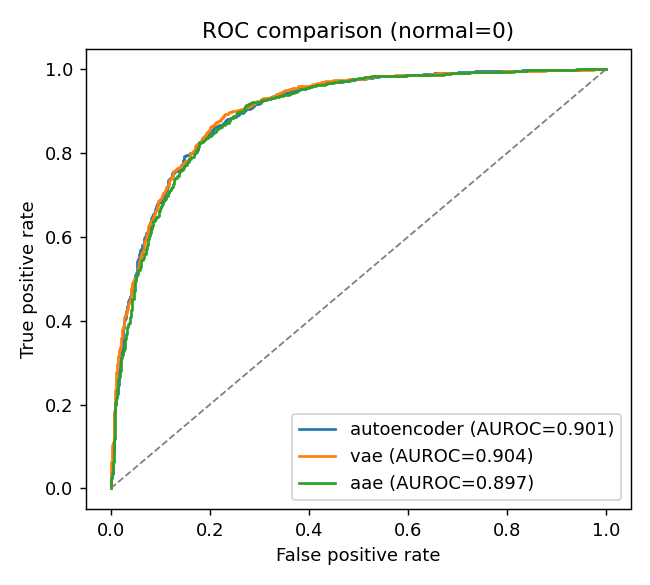
\includegraphics[width=0.48\textwidth]{figures/overlay_roc.png}
\hfill
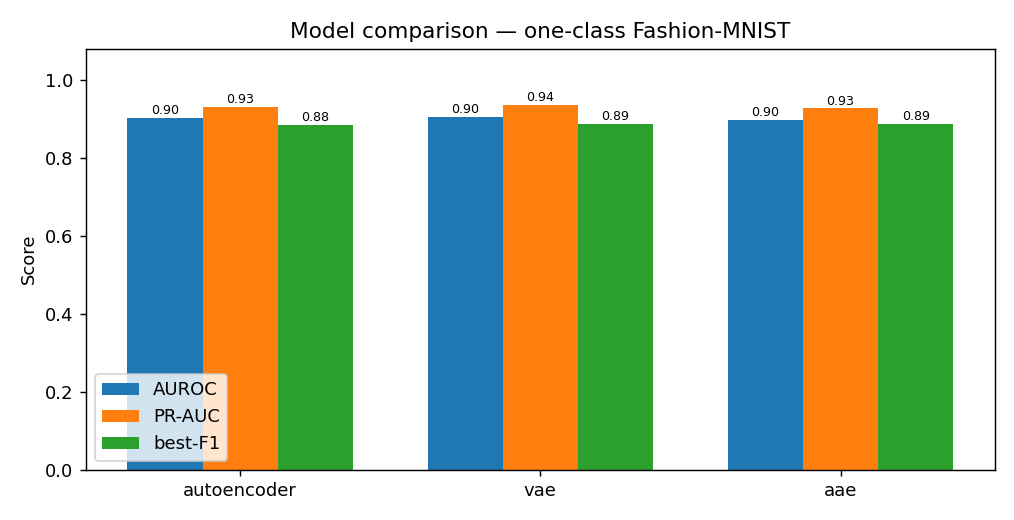
\includegraphics[width=0.48\textwidth]{figures/comparison_bars.png}
\caption{Left: ROC curves for the three models on the shared split, which nearly
overlap. Right: AUROC, PR-AUC, and best-F1 side by side. The visual near-overlap
mirrors the numeric near-tie in Table~\ref{tab:comparison}.}
\label{fig:comparison}
\end{figure}

Read along the latent-regularization spectrum, neither the explicit KL divergence
(VAE) nor the adversarial match (AAE) yields a clear improvement over the
unconstrained AE. This is consistent with the interpretation developed in the
Discussion: when the anomaly score is reconstruction error alone, a better-organised
latent space need not translate into a larger separation between normal and
anomalous reconstruction errors.

% =====================================================================
\section{Discussion and Limitations}   % [P1 — draft; all add a sentence]
% =====================================================================
The results show that reconstruction-based anomaly detection is effective on the
Fashion-MNIST one-class task: even the plain AE reaches strong, consistent
performance, confirming that learning to reconstruct normal data yields a useful
anomaly signal. The central question, however, was whether latent-space
regularization improves on that baseline, and the evidence is nuanced. The VAE
and AAE impose genuine structure on the latent space, yet their AUROC and PR-AUC
sit within roughly one percentage point of the AE (Table~\ref{tab:comparison}).
With single-seed point estimates and a margin this small, we treat the three
models as statistically indistinguishable on this benchmark rather than claiming
a strict ordering; establishing a reliable ranking would require multi-seed runs
with confidence intervals, which we identify as future work.

A natural explanation lies in the scoring rule. All three models are evaluated
with the same reconstruction-error score, which is exactly what makes the
comparison fair, but it also means the evaluation never directly consults the
latent probability (VAE) or the discriminator's judgment (AAE). A better-organised
latent space therefore need not translate into a larger gap between normal and
anomalous reconstruction errors. The $\beta$-VAE ablation supports this reading:
pushing the KL term harder measurably lowers AUROC, consistent with a
reconstruction--regularization trade-off in which an over-constrained latent
starts to cost the decoder information it needs to reconstruct even normal inputs.
The AAE exhibits an analogous tension between its reconstruction and adversarial
objectives.

The per-class AE results add a second axis of difficulty. Classes such as
Trouser, Sneaker, and Boot are easy because they are visually distinctive, whereas
Shirt is hard because it overlaps with T-shirt, Pullover, and Coat. This shows
that anomaly-detection difficulty depends on the visual distance between the
normal class and its anomalies as much as on the model.

Several limitations bound these conclusions. First, evaluation is image-level: the
models flag an anomalous image but do not localise the anomalous region, which
industrial settings often require. Second, Fashion-MNIST anomalies are other
clothing classes rather than genuine defects such as scratches or contamination.
Third, the results depend on hyperparameters --- latent dimension, learning rate,
epoch count, and regularization strength --- as the ablations directly show.
Fourth, the shared reconstruction-error score may under-represent the benefit of
the VAE's and AAE's structured latents, so latent-aware scores are the natural
next test. Fifth, adversarial (AAE) training is inherently less stable than plain
reconstruction training, although confining the game to the low-dimensional latent
makes it far more stable than image-space GAN training.

% =====================================================================
\section{Conclusion}   % [P1 — draft last]
% =====================================================================
This project compared three autoencoder-based generative models --- AE, VAE, and
AAE --- for one-class anomaly detection, arranged as a controlled spectrum of
latent-space regularization. By keeping the dataset, preprocessing, backbone,
scoring rule, and metrics fixed, the comparison isolates the effect of the
regularization mechanism itself. All three models achieve strong performance on
Fashion-MNIST: the AE baseline reaches approximately $0.90$ mean AUROC across all
ten classes, and on the shared T-shirt setup the VAE, AE, and AAE finish within
about one percentage point of one another. The main finding is therefore not that
the most complex model wins, but that latent-space regularization is a meaningful
design choice whose benefit depends on the scoring rule, the dataset's difficulty,
and the regularization strength --- a controlled scientific comparison rather than
a mere collection of implementations. Future work should evaluate on MVTec~AD with
pixel-level localization, run multi-seed experiments with error bars, and, most
directly, adopt latent-aware anomaly scores (reconstruction probability or
prior-distance) that better exploit the structured latents the VAE and AAE learn.

\begin{thebibliography}{9}
\bibitem{kingma2013} D.~P. Kingma and M.~Welling. Auto-Encoding Variational Bayes. ICLR, 2014.
\bibitem{ancho2015} J.~An and S.~Cho. Variational Autoencoder based Anomaly Detection using Reconstruction Probability. 2015.
\bibitem{makhzani2015} A.~Makhzani, J.~Shlens, N.~Jaitly, I.~Goodfellow, B.~Frey. Adversarial Autoencoders. 2015.
\bibitem{goodfellow2014} I.~Goodfellow et al. Generative Adversarial Nets. NeurIPS, 2014.
\bibitem{bergmann2019} P.~Bergmann et al. MVTec AD --- A Comprehensive Real-World Dataset for Unsupervised Anomaly Detection. CVPR, 2019.
\end{thebibliography}

\end{document}
